\documentclass[tikz, border=10pt]{standalone}
\usepackage{tikz}
\usetikzlibrary{arrows.meta, positioning, calc, shapes.geometric, decorations.pathreplacing}

% --- Professional Style Definitions ---
\tikzset{
	font=\sffamily\scriptsize,
	>=Stealth,
	% Actors
	actor/.style={draw, fill=blue!10, thick, minimum width=2.5cm, minimum height=0.8cm, rounded corners},
	% Lifelines
	lifeline/.style={draw, dashed, gray, thick},
	% Message Arrows
	msg/.style={->, thick, black},
	msglabel/.style={midway, above, font=\scriptsize, align=center},
	% Note boxes (delays, info)
	note/.style={fill=yellow!10, text=gray, font=\tiny, align=right, anchor=east},
	% Grouping Blocks (Echo, KEM)
	blockbox/.style={draw=gray, dashed, fill=gray!5, rounded corners},
	blocklabel/.style={anchor=north west, font=\bfseries\scriptsize, color=gray},
	% Critical Failure
	fail/.style={cross out, draw=red, thick, minimum size=5mm},
	% Defined the missing 'short' style
	short/.style={thick, -} 
}

\begin{document}
	
	% CHANGED: y=1cm (Positive Y goes UP) to match your coordinate logic
	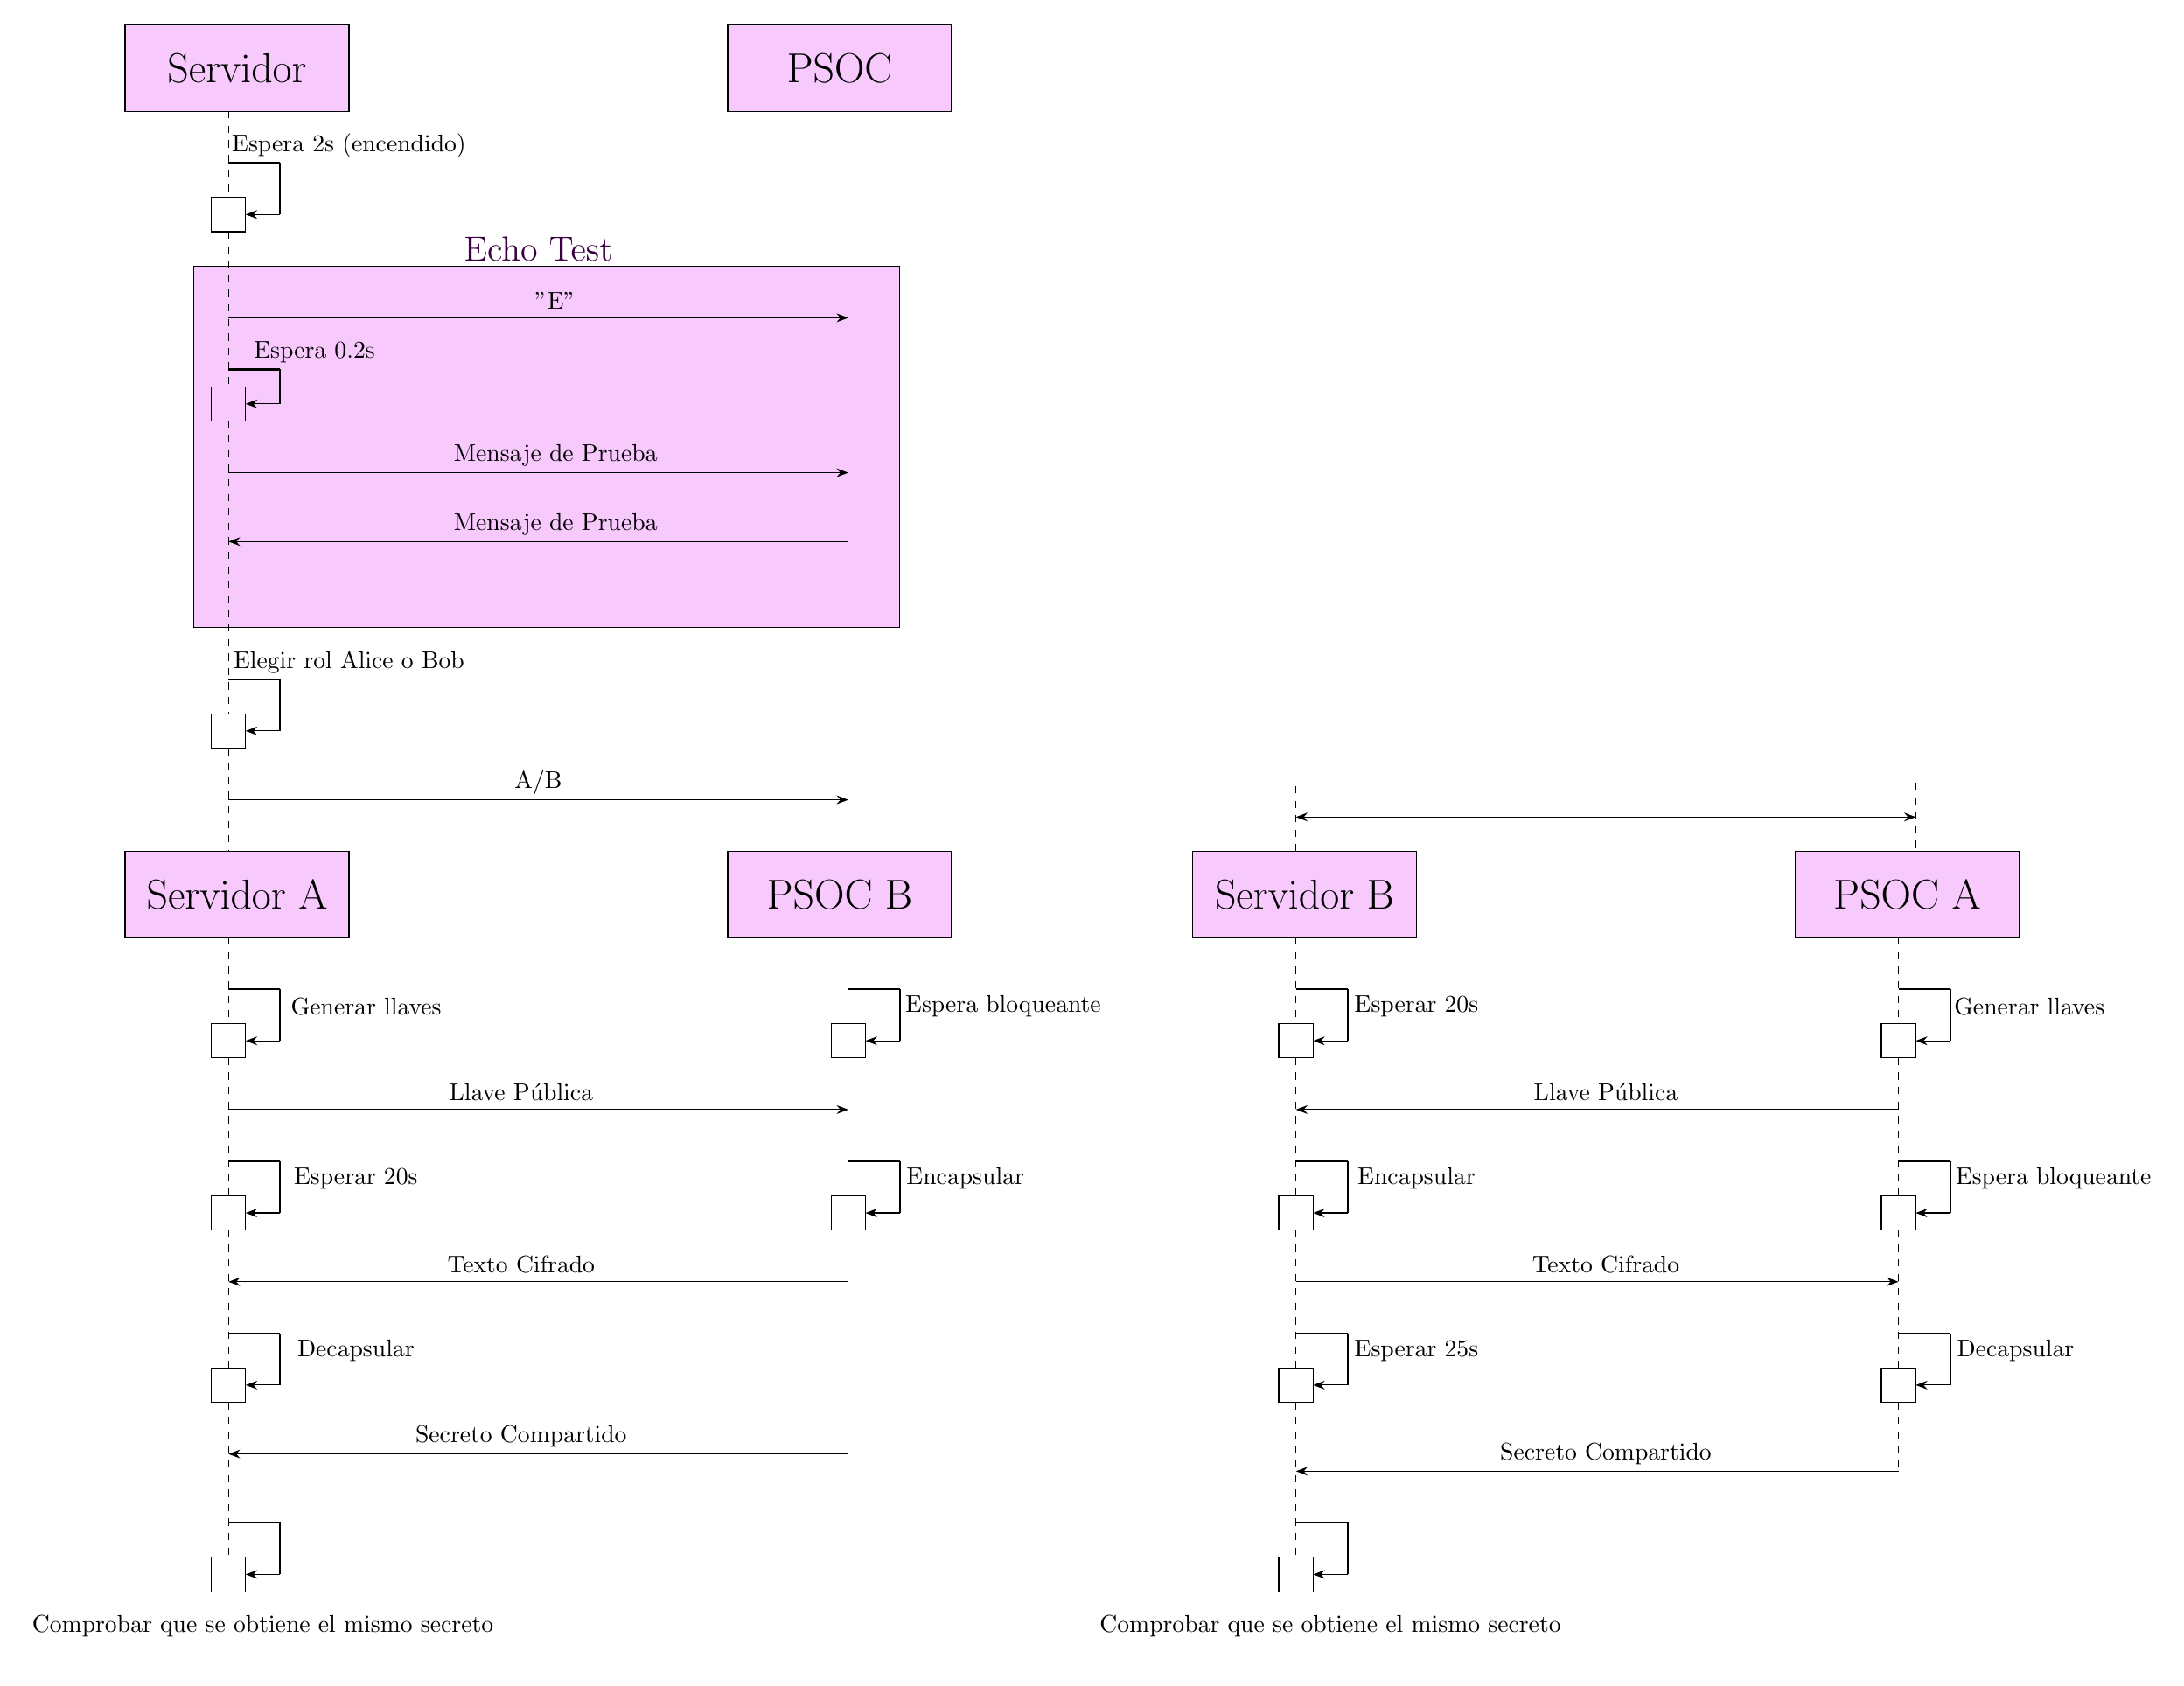
\begin{tikzpicture}[x=1cm, y=1cm] 
		
		\tikzstyle{every node}=[font=\normalsize]
		
		\draw [ fill={rgb,255:red,247; green,201; blue,253} ] (3.25,16.25) rectangle  node {\LARGE Servidor} (6.5,15);
		\draw [ fill={rgb,255:red,247; green,201; blue,253} ] (12,16.25) rectangle  node {\LARGE PSOC} (15.25,15);
		\draw  (6.25,14.75) rectangle (6.25,14.75);
		\draw  (6.5,14.75) rectangle (6.5,14.75);
		\draw [dashed] (4.75,15) -- (4.75,13.75);
		\node [font=\normalsize] at (6.5,14.5) {Espera 2s (encendido)};
		\draw  (4.5,13.75) rectangle (5,13.25);
		\draw [short] (4.75,14.25) -- (5.5,14.25);
		\draw [short] (5.5,14.25) -- (5.5,13.5);
		\draw [->, >=Stealth] (5.5,13.5) -- (5,13.5);
		\draw [ fill={rgb,255:red,247; green,201; blue,253} ] (4.25,12.75) rectangle (14.5,7.5);
		\node [font=\Large, color={rgb,255:red,59; green,0; blue,66}] at (9.25,13) {Echo Test};
		\draw [dashed] (4.75,13.25) -- (4.75,11);
		\draw [dashed] (13.75,15) -- (13.75,4.25);
		\draw [->, >=Stealth] (4.75,12) -- (13.75,12);
		\node [font=\normalsize] at (9.5,12.25) {"E"};
		\node [font=\normalsize] at (6,11.5) {Espera 0.2s};
		\draw  (4.5,11) rectangle (5,10.5);
		\draw [->, >=Stealth] (5.5,10.75) -- (5,10.75);
		\node [font=\normalsize] at (5.5,11) {};
		\draw [short] (4.75,11.25) -- (5.5,11.25);
		\node [font=\normalsize] at (6,13.25) {};
		\draw [short] (5.5,11.25) -- (5.5,10.75);
		\draw [dashed] (4.75,10.5) -- (4.75,6.25);
		\draw [->, >=Stealth] (4.75,9.75) -- (13.75,9.75);
		\node [font=\normalsize] at (9.5,10) {Mensaje de Prueba};
		\draw [->, >=Stealth] (13.75,8.75) -- (4.75,8.75);
		\node [font=\normalsize] at (9.5,9) {Mensaje de Prueba};
		\draw [dashed] (9.25,7.75) -- (9.25,7.75);
		\draw [dashed] (13.75,3) -- (13.75,1.75);
		\draw  (4.5,6.25) rectangle (5,5.75);
		\draw [->, >=Stealth] (5.5,6) -- (5,6);
		\node [font=\normalsize] at (5.5,6) {};
		\draw [short] (4.75,6.75) -- (5.5,6.75);
		\node [font=\normalsize] at (6.5,7) {Elegir rol Alice o Bob};
		\draw [short] (5.5,6.75) -- (5.5,6);
		\draw [ fill={rgb,255:red,247; green,201; blue,253} ] (3.25,4.25) rectangle  node {\LARGE Servidor A} (6.5,3);
		\draw [ fill={rgb,255:red,247; green,201; blue,253} ] (18.75,4.25) rectangle  node {\LARGE Servidor B} (22,3);
		\draw [dashed] (20.25,4.25) -- (20.25,5.25);
		\draw [dashed] (4.75,5.75) -- (4.75,4.25);
		\draw [dashed] (4.75,3) -- (4.75,1.75);
		\draw [dashed] (20.25,3) -- (20.25,1.75);
		\draw  (4.5,1.75) rectangle (5,1.25);
		\node [font=\normalsize] at (5.75,5.5) {};
		\node [font=\normalsize] at (6,5.75) {};
		\node [font=\normalsize] at (5.75,6) {};
		\node [font=\normalsize] at (6.25,1) {};
		\node [font=\normalsize] at (6.5,1.25) {};
		\node [font=\normalsize] at (6.75,2) {Generar llaves};
		\draw [short] (4.75,2.25) -- (5.5,2.25);
		\draw [short] (5.5,2.25) -- (5.5,1.5);
		\draw [->, >=Stealth] (5.5,1.5) -- (5,1.5);
		\draw [dashed] (4.75,1.25) -- (4.75,-0.75);
		\draw [->, >=Stealth] (4.75,0.5) -- (13.75,0.5);
		\node [font=\normalsize] at (9,0.75) {Llave Pública};
		\draw [->, >=Stealth] (4.75,5) -- (13.75,5);
		\node [font=\normalsize] at (9.25,5.25) {A/B};
		\draw [ fill={rgb,255:red,247; green,201; blue,253} ] (12,4.25) rectangle  node {\LARGE PSOC B} (15.25,3);
		\draw [ fill={rgb,255:red,247; green,201; blue,253} ] (27.5,4.25) rectangle  node {\LARGE PSOC A} (30.75,3);
		\draw [short] (13.25,16.25) -- (13.25,16.25);
		\draw [short] (21.25,14.5) -- (21.25,14.5);
		\draw [dashed] (29.25,5.25) -- (29.25,4.25);
		\draw [dashed] (29,3) -- (29,1.75);
		\node [font=\normalsize] at (5.75,1) {};
		\node [font=\normalsize] at (5.25,1) {};
		\node [font=\normalsize] at (5.75,1.75) {};
		\node [font=\normalsize] at (5.75,1) {};
		\node [font=\normalsize] at (6,1.5) {};
		\node [font=\normalsize] at (5.75,1.75) {};
		\node [font=\normalsize] at (5.75,1.75) {};
		\draw [short] (4.75,0) -- (4.75,0);
		\draw [short] (4.75,-0.25) -- (5.5,-0.25);
		\draw [short] (13.75,-0.25) -- (14.5,-0.25);
		\draw [short] (20.25,-0.25) -- (21,-0.25);
		\draw [short] (29,-0.25) -- (29.75,-0.25);
		\draw [short] (13.75,2.25) -- (14.5,2.25);
		\draw [short] (14.5,2.25) -- (14.5,1.5);
		\draw [short] (20.25,2.25) -- (21,2.25);
		\draw [short] (21,2.25) -- (21,1.5);
		\draw [short] (29,2.25) -- (29.75,2.25);
		\draw [short] (29.75,2.25) -- (29.75,1.5);
		\draw [short] (5.5,-0.25) -- (5.5,-1);
		\draw [short] (14.5,-0.25) -- (14.5,-1);
		\draw [short] (21,-0.25) -- (21,-1);
		\draw [short] (29.75,-0.25) -- (29.75,-1);
		\draw  (4.5,-1.25) rectangle (5,-0.75);
		\draw  (13.5,-0.75) rectangle (14,-1.25);
		\draw  (20,-0.75) rectangle (20.5,-1.25);
		\draw  (28.75,-0.75) rectangle (29.25,-1.25);
		\draw  (13.5,1.75) rectangle (14,1.25);
		\draw  (20,1.75) rectangle (20.5,1.25);
		\draw  (28.75,1.75) rectangle (29.25,1.25);
		\draw [->, >=Stealth] (14.5,1.5) -- (14,1.5);
		\draw [->, >=Stealth] (21,1.5) -- (20.5,1.5);
		\draw [->, >=Stealth] (29.75,1.5) -- (29.25,1.5);
		\draw [->, >=Stealth] (14.5,-1) -- (14,-1);
		\draw [->, >=Stealth] (21,-1) -- (20.5,-1);
		\draw [->, >=Stealth] (29.75,-1) -- (29.25,-1);
		\draw [dashed] (13.75,1.25) -- (13.75,-0.75);
		\draw [dashed] (20.25,1.25) -- (20.25,-0.75);
		\draw [dashed] (29,1.25) -- (29,-0.75);
		\node [font=\normalsize] at (16,2) {Espera bloqueante};
		\node [font=\normalsize] at (30.9,2) {Generar llaves};
		\node [font=\normalsize] at (22,2) {Esperar 20s};
		\draw [->, >=Stealth] (29,0.5) -- (20.25,0.5);
		\node [font=\normalsize] at (24.75,0.75) {Llave Pública};
		\draw [->, >=Stealth] (5.5,-1) -- (5,-1);
		\node [font=\normalsize] at (6.6,-0.5) {Esperar 20s};
		\draw [<->, >=Stealth] (20.25,4.75) -- (29.25,4.75);
		\node [font=\normalsize] at (31.25,-0.5) {Espera bloqueante};
		\node [font=\normalsize] at (15.45,-0.5) {Encapsular};
		\node [font=\normalsize] at (22,-0.5) {Encapsular};
		\draw [dashed] (4.75,-1.25) -- (4.75,-3.25);
		\draw [dashed] (13.75,-1.25) -- (13.75,-4.5);
		\draw [dashed] (20.25,-1.25) -- (20.25,-3.25);
		\draw [dashed] (29,-1.25) -- (29,-3.25);
		\draw [->, >=Stealth] (13.75,-2) -- (4.75,-2);
		\draw [->, >=Stealth] (20.25,-2) -- (29,-2);
		\node [font=\normalsize] at (9,-1.75) {Texto Cifrado};
		\node [font=\normalsize] at (24.75,-1.75) {Texto Cifrado};
		\draw [short] (4.75,-2.75) -- (5.5,-2.75);
		\draw [short] (20.25,-2.75) -- (21,-2.75);
		\draw [short] (29,-2.75) -- (29.75,-2.75);
		\draw [short] (29.75,-2.75) -- (29.75,-3.5);
		\draw [short] (21,-2.75) -- (21,-3.5);
		\draw [short] (5.5,-2.75) -- (5.5,-3.5);
		\draw  (4.5,-3.25) rectangle (5,-3.75);
		\draw  (20,-3.25) rectangle (20.5,-3.75);
		\draw  (28.75,-3.25) rectangle (29.25,-3.75);
		\draw [->, >=Stealth] (5.5,-3.5) -- (5,-3.5);
		\draw [->, >=Stealth] (21,-3.5) -- (20.5,-3.5);
		\draw [->, >=Stealth] (29.75,-3.5) -- (29.25,-3.5);
		\node [font=\normalsize] at (6.6,-3) {Decapsular};
		\node [font=\normalsize] at (22,-3) {Esperar 25s};
		\node [font=\normalsize] at (30.7,-3) {Decapsular};
		\draw [dashed] (4.75,-3.75) -- (4.75,-6);
		\draw [dashed] (20.25,-3.75) -- (20.25,-6);
		\draw [dashed] (29,-3.75) -- (29,-4.75);
		\draw [->, >=Stealth] (13.75,-4.5) -- (4.75,-4.5);
		\node [font=\normalsize] at (9,-4.25) {Secreto Compartido};
		\draw [->, >=Stealth] (29,-4.75) -- (20.25,-4.75);
		\node [font=\normalsize] at (24.75,-4.5) {Secreto Compartido};
		\draw [short] (20.25,-5.5) -- (21,-5.5);
		\draw [short] (21,-5.5) -- (21,-6.25);
		\draw  (20,-6) rectangle (20.5,-6.5);
		\draw [->, >=Stealth] (21,-6.25) -- (20.5,-6.25);
		\draw  (5,-6) rectangle (4.5,-6.5);
		\draw [short] (4.75,-5.5) -- (5.5,-5.5);
		\draw [short] (5.5,-5.5) -- (5.5,-6.25);
		\draw [->, >=Stealth] (5.5,-6.25) -- (5,-6.25);
		\node [font=\normalsize] at (5.25,-7) {Comprobar que se obtiene el mismo secreto};
		\node [font=\normalsize] at (20.75,-7) {Comprobar que se obtiene el mismo secreto};
		\draw [dashed] (19.75,-7.5) -- (19.75,-7.5);
		
	\end{tikzpicture}
	
\end{document}